\section*{Multi-Carrier and OFDM Technologies}






La tecnologia multi-carrier è impiegata da tutte le modulazioni più recenti e rappresenta la base del livello fisico per trasmissioni LTE, 5G e Wi-Fi. 
L'ampio utilizzo di questa tiplogia di modulazione deriva dalla capacità di ridurre i problemi derivanti dall'utilizzo di un canale frequency selective, i cui problemi sono sempre più evidenti all'aumentare del rate di trasmissione. 
Inoltre presenta dei benefici anche nell'occupazione spettrale e nella flessibilità di allocazione delle risorse radio ai vari utenti del sistema.
\begin{itemize}
    \item Robustezza contro canali frequecy-selective
    \item Efficienza spettrale
    \item Allocazione flessibile di risorse
\end{itemize}

L'idea base consiste nel suddividere il segnale originale da trasmettere, caratterizzato da una banda ben superiore rispetto alla coherence bandwidth del canale in tanti segnali,
ciascuno avente una banda tale da evitare i problemi del canale frequency selective, ovvero inferiori alla coherence bandwidth.


\begin{center}
    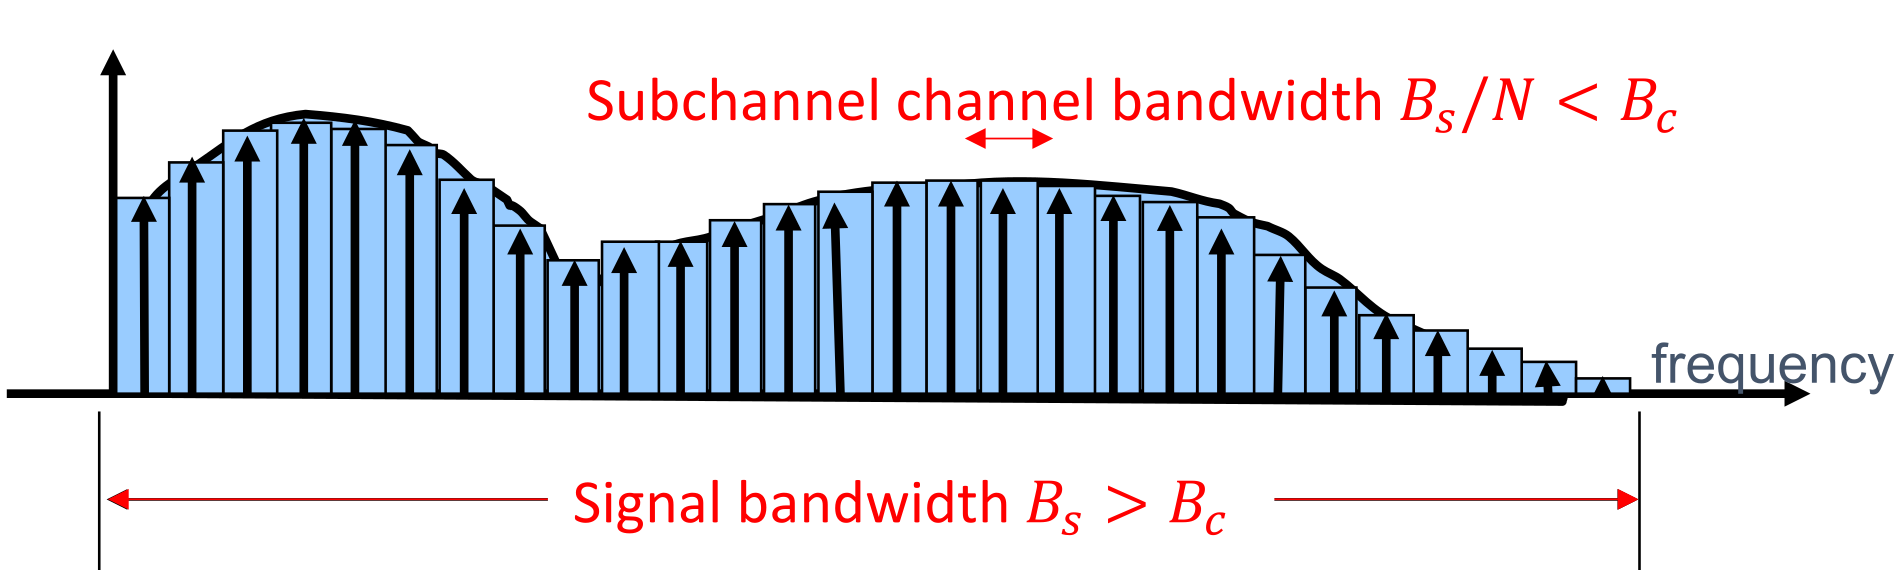
\includegraphics[width=0.8\textwidth]{imgs/multicarrier.jpg}
\end{center}

\[
  B_s > B_c \Rightarrow \text{frequency selective channel}  
\]

\[
    \Delta B = \frac{B_s}{N} < B_c \Rightarrow \text{flat fading channel}
\]
I segnali in cui è stato suddiviso l'originale non saranno affetti da ISI.
Per effettuare una trasmissione parallela dei vari segnali si potrebbe utilizzare filtri passa banda in parallelo, tuttavia nella pratica cioè non è possibile a causa della mancanza di un filtro ideale, la cui rappresentazione in frequenza sarebbe una perfetta rect. Inoltre l'utilizzo di molti filtri sarebbe molto costoso.


\begin{center}
    \resizebox{0.5\textwidth}{!}{
        \begin{tikzpicture}[
                block/.style={rectangle, draw, minimum height=1cm, minimum width=1.5cm},
                node distance=1cm and 1cm,
                auto,
                every node/.style={align=center}
            ]
            \newcommand{\signalshapee}{
                \draw (-0.5, -0.25) -- (-0.35, -0.25) -- (-0.35, 0.25) -- (-0.25, 0.25) -- (-0.25, -0.25) -- (0.5, -0.25); 
            }


            \newcommand{\signalshape}{
                    \draw (-0.5, -0.25) -- (-0.25, -0.25) -- (-0.25, 0.25) -- (-0.15, 0.25) -- (-0.15, -0.25) -- (0.5, -0.25); 
            }
            \newcommand{\signalshapeeee}{
                \draw (-0.5, -0.25) -- (0.15, -0.25) -- (0.15, 0.25) -- (0.25, 0.25) -- (0.25, -0.25) -- (0.5, -0.25); 
            }

            \newcommand{\signalshapeee}{
                \draw (-0.5, -0.25) -- (0.25, -0.25) -- (0.25, 0.25) -- (0.35, 0.25) -- (0.35, -0.25) -- (0.5, -0.25);
            }
        
            \node[block] (encoder) {Source};
            \node[block, right=of encoder, inner sep=0pt, minimum size=0pt] (interp) {};

            \node[above=2cm of interp, inner sep=0pt, minimum size=0pt] (dummy1) {};
            \node[above=3.5cm of dummy1, inner sep=0pt, minimum size=0pt] (dummy2) {};
            \node[below=2cm of interp, inner sep=0pt, minimum size=0pt] (dummy_1) {};
            \node[below=3.5cm of dummy_1, inner sep=0pt, minimum size=0pt] (dummy_2) {};

            \node[block, right=1.5cm of dummy1, path picture={ % Use path picture to embed another TikZ graphic
            \begin{scope}[shift={(path picture bounding box.center)}]
                \signalshape
            \end{scope}
            }] (p1) {};
            \node[block, right=1.5cm of dummy2, path picture={ % Use path picture to embed another TikZ graphic
            \begin{scope}[shift={(path picture bounding box.center)}]
                \signalshapee
            \end{scope}
            }] (p2) {};
            \node[block, right=1.5cm of dummy_1, path picture={ % Use path picture to embed another TikZ graphic
            \begin{scope}[shift={(path picture bounding box.center)}]
                \signalshapeeee
            \end{scope}
            }] (p_1) {};
            \node[block, right=1.5cm of dummy_2, path picture={ % Use path picture to embed another TikZ graphic
            \begin{scope}[shift={(path picture bounding box.center)}]
                \signalshapeee
            \end{scope}
            }] (p_2) {};

            % create a dotted line between p1 and p_1
            \draw[line width=1pt,dash pattern=on 1pt off 15pt] (p1) -- (p_1);

            \node[draw, circle, right=2cm of p1] (m1) {\(\times\)}; 
            \node[draw, circle, right=2cm of p2] (m2) {\(\times\)};
            \node[draw, circle, right=2cm of p_1] (m_1) {\(\times\)};
            \node[draw, circle, right=2cm of p_2] (m_2) {\(\times\)};

            \draw[->] (p1) -- (m1);
            \node[below=of m1] (cos) {$e^{j2\pi (f_1 + \Delta f) t}$};
            \draw[->] (cos) -- (m1);

            \draw[->] (p2) -- (m2);
            \node[below=of m2] (sin) {$e^{j2\pi f_1 t}$};
            \draw[->] (sin) -- (m2);

            \draw[->] (p_1) -- (m_1);
            \node[below=of m_1] (coss) {$e^{j2\pi (f_1 + (N - 2) \Delta f) t}$};
            \draw[->] (coss) -- (m_1);


            \draw[->] (p_2) -- (m_2);
            \node[below=of m_2] (sinn) {$e^{j2\pi (f_1 + (N - 1) \Delta f) t}$};
            \draw[->] (sinn) -- (m_2);

            \node[right=2cm of m1, inner sep=0pt, minimum size=0pt] (dummy3) {};
            \node[right=2cm of m2, inner sep=0pt, minimum size=0pt] (dummy4) {};

            
            \node[draw, circle, right=7.5cm of interp] (sum) {\(+\)};

            \draw[->] (m1) -| (sum);
            \draw[->] (m2) -| (sum);
            
            \draw[->] (m_1) -| (sum);
            \draw[->] (m_2) -| (sum);

            \node[right=2cm of sum] (dummy5) {};
            \draw[->] (sum) -- node[midway, above] {$s(t)$} (dummy5) {};


            \draw[->] (interp) |- node[midway, above] {} (p1);
            \draw[->] (interp) |- node[midway, below] {} (p2);
            \draw[->] (interp) |- node[midway, above] {} (p_1);
            \draw[->] (interp) |- node[midway, below] {} (p_2);

            \draw[->] (encoder) -- (interp) node[midway,above] {};


        \end{tikzpicture}
    }
\end{center}
Per poter analizzare una modulazione multi-carrier è necessaria una rappresentazione alternativa, ma equivalente, del canale di trasmissione, ottenuta campionando il segnale con frequenza $\frac{1}{T}$. La rappresentazione ottenuta risulta valida solo nella banda del segnale trasmesso, ma non è un problema dato che non si ha interesse nell'analizzare il canali in altri punti.

Considerando l'inviluppo complesso risulta chiaro che la condizione di Nyquist\footnote{\label{nyquist_cond} La condizione di Nyquist garantisce l'assenza di aliasing per segnali campionati, ovvero dato l'intervallo di campionamento $T_s$ e la banda $B$ del segnale da campionare, deve valere $T_s \leq \frac{1}{2B}$, ovvero $f_s \geq 2B$} è rispettata con frequenza di campionamente $\frac{1}{T}$.



\[
    f_s \geq 2 \frac{1}{2T} = \frac{1}{T} \quad \text{frequenza di campionamento} 
\]
\[
    h_{eq}(t) = \sum_{\ell=0}^{L-1} h \left[\ell\right] \delta(t - \ell T) \quad \text{rappresentazione equivalente del canale}
\]

\[
    y(t) = h_{eq}(t) \ast s(t) = \sum_{\ell=0}^{L-1} h\left[\ell\right] s(t - \ell T) \quad \text{inviluppo complesso del segnale ricevuto}
\]

Dove $h_{eq}$ è la rappresentazione equivalente del canale, che si può sempre ottenere dalla formula del canale $ h(t) = A_{LS} \sum_{\ell=0}^{N_c-1} \alpha_{\ell} e^{j\phi_{\ell}} \delta(t - \tau_{\ell})$, dove nella versione equivalente il segnale è campionato a multipli di $T$.

Il segnale ricevuto è identico al segnale ottenuto utilizzando la rappresentazione fisica del canale, ma la forma permette un'analisi più semplice.
\subsection*{Cenni sulla trasformata discreta di Fourier}
Una sequenza \( x[n] \) è \textit{periodica} se esiste un intero positivo $N_0$ (il \textit{periodo} della sequenza) per il quale è verificata la seguente relazione:
\[
    x[n] = x[n + N_0] \quad \forall n
\]
Supponiamo che il periodo di ripetizione $T_0$ e l'intervallo di campionamento $T$ siano in relazione:
\[
    N_0 T = T_0
\]
e cerchiamone la relazione con $x(t)$, considerando la sua equazione di sintesi:

\[
    x(t) = \sum_{k=-\infty}^{\infty} X_k e^{j2\pi k f_0 t}
\]
dalla quale ricaviamo il campione
\[
    x[n] = x(nT) = \sum_{k=-\infty}^{\infty} X_k e^{\frac{j2\pi k nT}{T_0}} = \sum_{k=-\infty}^{\infty} X_k e^{\frac{j2\pi k n}{N_0}}
\]
spezziamo la sommatoria, associando gli elementi all'interno di intervalli della forma $\rinterval{m\, N_0}{(m+1) N_0}$
\[
    x[n] = \sum_{m=-\infty}^{+\infty} \sum_{h=0}^{N_0-1} X_{mN_0 + h} e^{\frac{j2\pi (mN_0 + h) n}{N_0}} = \sum_{h=0}^{N_0-1} \left( \sum_{m=-\infty}^{+\infty} X_{mN_0 + h}\right) e^{\frac{j2\pi h n}{N_0}} = \sum_{h=0}^{N_0-1} \overline{X}_h e^{\frac{j2\pi h n}{N_0}} 
\]
avendo definito $\overline{X}_h = \sum_{m=-\infty}^{+\infty} X_{mN_0 + h}$, da ciò possiamo arrivare alle seguenti relazioni:
\[
    x[k] = \sum_{k=0}^{N-1} \overline{X}_k e^{\frac{j2\pi kn}{N}} \quad \text{anti-trasformata discreta di Fourier}
\]
\[
    \overline{X}_k = \frac{1}{N} \sum_{k=0}^{N-1} x[k] e^{-\frac{j2\pi kn}{N}} \quad \text{trasformata discreta di Fourier}
\]
In particolare, la DFT verrà utilizzata per convertire una collezione finita di campioni equispaziati di una funzione in una collezione di coefficienti di una combinazione lineare di sinusoidi complesse,
assumendo implicitamente che la funzione sia periodica con periodo pari alla lunghezza della sequenza di campioni, per motivi non chiari al sottoscritto.
\subsection*{Modulazione OFDM}
La modulazione OFDM risulta essere una delle più utilizzate per trasmissioni digitali ed è del tipo multi-carrier, ereditando quindi i vantaggi di tale tipo di modulazione.
Si consideri un blocco $S$ composto da $N$ campioni da trasmettere:
\[
  S = \left\{s\left[0\right], s\left[1\right], \ldots, s\left[N-1\right]\right\}
\]
L'effetto introdotto dal canale genera una componente ISI lato ricevitore:
\[
  y\left[k\right] = \sum_{\ell=0}^{L-1} h\left[\ell\right] s\left[k - \ell\right] = h(0)s\left[k\right] + \sum_{\ell=1}^{L-1} h\left[\ell\right] s\left[k - \ell\right]
\]
Tipicamente quando si studia una modulazione si considera una sequenza infinita di simboli, ma in questo caso se ne considera una di $N$ simboli, quindi gli indici negativi vengono considerati come 0 dato che non esistono.

% create a system of equations
%\[
%  \begin{cases}
%    y(0) = h(0)s(0) \\
%    y(1) = h(0)s(1) + h(1)s(0) \\
%    \vdots \\
%    y(N-1) = h(0)s(N-1) + h(1)s(N-2) + \ldots + h(L-1)s(N-L)
%  \end{cases}
%\]

% inset square brackets
\[
    \begin{cases}
        y[0] = h[0]s[0] \\
        y[1] = h[0]s[1] + h[1]s[0] \\
        \vdots \\
        y[N-1] = h[0]s[N-1] + h[1]s[N-2] + \ldots + h[L-1]s[N-L]
    \end{cases}
\]

Ovvero possiamo anche riscrivere il segnale ricevuto come:
\[
y[k] = \sum_{\ell=0}^{\min(L-1, k)} h[\ell] s[k-\ell]
\]


L'espressione può essere riscritta in forma matriciale: $\mathbf{y} = \mathbf{H} \mathbf{s}$, con $\mathbf{H} \in \mathbb{C}^{N \times N}$ 

\[ 
\begin{bmatrix} y[0] \\ y[1] \\ \vdots \\ y[N-1] \end{bmatrix} 
= 
\begin{bmatrix}
    h[0] & 0 & \cdots & \cdots & \cdots & \cdots & \cdots & 0 \\
    h[1] & h[0] & \cdots & 0 \\
    \vdots & \vdots & \ddots & \vdots \\
    h[L-1] & h[L-2] & \cdots & h[0] & 0 & \cdots & \cdots & 0 \\
    0 & h[L-1] & \cdots & h[1] & h[0] & 0 & \cdots & 0 \\
    \vdots & \vdots & \ddots & \vdots & \vdots \\
    0 & 0 & \cdots & h[L-1] & h[L-2] & \cdots & h[1] & h[0]
\end{bmatrix}   
\begin{bmatrix} s[0] \\ s[1] \\ \vdots \\ s[N-1] \end{bmatrix}
\]

La matrice $\mathbf{H}$ è detta \textbf{matrice di Toeplitz} e la sua proprietà caratteristica è la presenza del solito elemento lungo le diagonali. Copiando gli ultimi $N_{CP} > L$ campioni del blocco $S$ e appendendoli in testa si ottiene un nuovo blocco con struttura circolare, cioè i primi $N_{CP}$ campioni sono identici agli ultimi $N_{CP}$.
\[
    \overline{S} = \left\{s\left[N - N_{CP} - 1\right], \ldots, s\left[N - 1\right], s\left[0\right], \ldots, s\left[N - 1\right]\right\} \quad \text{blocco cliclico}
\]


Il prefisso appeso in testa può essere utilizzato come elementi con indice negativo nella convuluzione con il canale.

%\[
%    \overline{S}(-1) = S(N - 1)
%\]
%\[
%    \overline{S}(-2) = S(N - 2)
%\]
%\[
%    \vdots
%\]
%\[
%    \overline{S}(-N_{CP}) = S(N - N_{CP})
%\]


\[
    \begin{array}{ll}
        \overline{s}[-1] = s[N - 1] \\
        \overline{s}[-2] = s[N - 2] \\
        \vdots \\
        \overline{s}[-N_{CP}] = s[N - N_{CP}]
    \end{array}
\]



Calcolando nuovamente la convoluzione, adesso ogni campione avrà anche alcune componenti con indice negativo.
Introducendo il prefisso nel blocco trasmesso in uscita dal canale si ottiene un vettore $\mathbf{y}$ i cui elementi sono costituiti dalla somma di $L$ termini.
\[
y[k] = \sum_{\ell=0}^{L-1} h[\ell] s[(k-\ell) \mod N]
\]
Ovvero:

\[
    y[k] = \sum_{\ell=0}^{L-1} h[\ell] \ \overline{s}[k-\ell]
\]
Che può anche essere espressa, per risaltare la componente aggiuntiva rispetto all'idea iniziale, come:
\[
y[k] = \sum_{\ell=0}^{\min(L-1, k)} h[\ell] s[k-\ell] + \sum_{\ell=\min(L-1, k)+1}^{L-1} h[\ell] s[k-\ell + N]
\]
In forma matriciale diventa:
\[
    \mathbf{y} = \mathbf{\overline{H}} \mathbf{s}
\]
Invece di aggiungere elementi al vettore $\mathbf{s}$, ottentendo un vettore $\mathbf{\overline{s}}$, si modifica la matrice $\mathbf{H}$.
\[ 
\begin{bmatrix} y[0] \\ y[1] \\ \vdots \\ y[N-1] \end{bmatrix} 
= 
\begin{bmatrix}
    h[0] & 0 & \cdots & \cdots & \cdots & h[3] & h[2] & h[1] \\
    h[1] & h[0] & \cdots & 0 & \cdots & h[4] & h[3] & h[2] \\
    \vdots & \vdots & \ddots & \vdots & &  & \vdots & \vdots \\
    h[L-1] & h[L-2] & \cdots & h[0] & 0 & \cdots & 0 & 0 \\
    0 & h[L-1] & \cdots & h[1] & h[0] & 0 & \cdots & 0 \\
    \vdots & \vdots & \ddots & \vdots & \vdots & & h[0] & 0 \\
    0 & 0 & \cdots & h[L-1] & h[L-2] & \cdots & h[1] & h[0]
\end{bmatrix}   
\begin{bmatrix} s[0] \\ s[1] \\ \vdots \\ s[N-1] \end{bmatrix}
\]



La nuova matrice risulta ancora essere del tipo Toeplitz, ma in aggiunta è anche \textbf{circolante}, dato che ogni riga è ottenuta tramite uno shift circolare verso destra della riga precedente (vale anche per le colonne, shiftando verso il basso).
Ogni matrice circolante può essere diagonalizzata, e in particolare può essere espressa come:
\[
    \overline{\mathbf{H}} = \mathbf{F}^H \mathbf{H} \mathbf{F}
\]




\[
    \begin{cases*}
        \mathbf{F}: \mathbf{F}_{n, m} = \frac{1}{\sqrt{N}} e^{\frac{-j2\pi nm}{N}} \quad \text{fourier trasform matrix normalizzata} \\
        \mathbf{H}: \mathbf{H}_{n, m} = \begin{cases*}
                                                        \sum_{\ell=0}^{N-1} h(\ell) e^{\frac{-j2\pi \ell n}{N}} & \text{se } $n = m$ \\
                                                        0 & \text{se } $n \neq m$
                                                    \end{cases*}
    \end{cases*}
\]
L'elemento $n$-esimo sulla diagonale risulta avere la trasformata  discreta di Fourier del canale (manca solo il termine $\frac{1}{\sqrt{N}}$)


La matrice $\mathbf{F}$ è unitaria, ovvero gode delle proprietà:
\begin{itemize}
    \item $\mathbf{F}^H \mathbf{F} = \mathbf{F} \mathbf{F}^H = \mathbf{I}_N$
    \item $\| \mathbf{F} \| = 1$ 
\end{itemize}

Considerando $\mathcal{F}\{\mathbf{y}\} = \mathbf{F} \mathbf{y}$ e $\mathbf{S} = \mathbf{F} \mathbf{s}$, ovvero le DFT dei due vettori si ottiene la seguente espresione:
\[
    \mathcal{F}\{\mathbf{y}\} = \mathbf{F} \mathbf{y} = \mathbf{F} \mathbf{\overline{H}} \mathbf{s} = \mathbf{F} \left(\mathbf{F}^H \mathbf{H} \mathbf{F}\right)\mathbf{s} =  \mathbf{H} \mathbf{F} \mathbf{s} = \mathbf{H} \mathcal{F}\{\mathbf{s}\}
\]
\[
    \Rightarrow \mathcal{F}\{\mathbf{y}\}_{n} = \mathbf{H}_{n,n} \mathcal{F}\{\mathbf{s}\}_{n} \quad \text{per } n = 0, 1, \ldots, N-1
\]
Dato che $\mathbf{H}$ è diagonale, il segnale ricevuto sul subcarrier $n$ dipende esclusivamente dal segnale trasmesso sullo stesso subcarrier. Nel dominio della frequenza quindi non abbiamo ISI.


\begin{center}
    \resizebox{\textwidth}{!}{
        \begin{tikzpicture}[
            block/.style={rectangle, draw, minimum height=1cm, minimum width=2.5cm},
            node distance=1cm and 2cm,
            align=center,
            auto
        ]
        \node[block] (BitSource) {Bit source};
        \node[block, right=of BitSource] (SymbolMapping) {Symbol\\mapping};
        \node[block, right=of SymbolMapping] (S2PConverter) {Serial\\to\\parallel\\converter};

        \node[block, right=of S2PConverter] (InverseDFT) {Inverse\\DFT};
        \node[block, right=of InverseDFT] (CpInsertion) {CP\\insertion};
        \node[right=of CpInsertion, inner sep=0pt, minimum size=0pt] (channel) {};

        \node[block, below=of channel] (MultipathChannel) {Multipath\\channel};

        \node[below=of MultipathChannel, inner sep=0pt, minimum size=0pt] (dummy2) {};
        \node[block, left=of dummy2] (CpRemoval) {CP\\removal};
        \node[block, left=of CpRemoval] (P2SConverter) {Serial\\to\\parallel\\converter};
        \node[block, left=of P2SConverter] (DFT) {DFT};
        \node[block, left=of DFT] (SymbolDecision) {Symbol\\decision};
        \node[block, left=of SymbolDecision] (Destination) {Destination};

        \draw[->] (BitSource) -- (SymbolMapping) node[midway,above] {$b[n]$};
        \draw[->] (SymbolMapping) -- (S2PConverter) node[midway,above] {};
        \draw[->] (S2PConverter) -- (InverseDFT) node[midway,above] {$\mathcal{F}\{\mathbf{s}\}$};
        \draw[->] (InverseDFT) -- (CpInsertion) node[midway,above] {$\mathbf{s}$};

        \draw[-] (CpInsertion) -- (channel) node[midway,above] {$\overline{\mathbf{s}}$};
        \draw[->] (channel) -- (MultipathChannel) node[midway,right] {};
        \draw[-] (MultipathChannel) -- (dummy2) node[midway,right] {};
        \draw[->] (dummy2) -- (CpRemoval) node[midway,above] {$\overline{\mathbf{y}}$};
%        % TODO: 2 Y uguali?
        \draw[->] (CpRemoval) -- (P2SConverter) node[midway,above] {$\mathbf{y}$};
        \draw[->] (P2SConverter) -- (DFT) node[midway,above] {};
        \draw[->] (DFT) -- (SymbolDecision) node[midway,above] {$\mathcal{F}\{\mathbf{y}\}$};
        \draw[->] (SymbolDecision) -- (Destination) node[midway,above] {$\hat{b}[n]$};
        \end{tikzpicture}
    }
\end{center}

%\draw[dashed, red, thick] ([xshift=-0.5cm,yshift=0.5cm]sampler.north west) rectangle ([xshift=0.5cm,yshift=-0.5cm]filter.south east);

%\node[align=center, red, above right= -1cm and -6cm of filter.south east] (channel-label) {Demodulatore numerico};


I simboli trasmessi sono idealmente generati in frequenza, ovvero sono convoluti prima della trasmissione tramite DFT inversa, quindi per essere recuperati è necessario effettuare la DFT. L'uso del prefisso risulta comunque essenziale affinché le proprietà algebriche sfruttate siano verificate. 
La DFT può essere calcolata tramite FFT, un'operazione molto semplice dato che è costituita da una moltiplicazione matriciale, quindi il costo per la rimozione dell'ISI è molto contenuto. In questo modo è vicino il limite del rate di tramissione raggiungibile, a patto che vi sia una banda sufficientemente ampia.
Il costo da pagare è l'utilizzo aggiuntivo di energia e banda per la trasmissione del prefisso, il quale non contiene alcuna informazione utile.
La denominazione OFDM deriva dal fatto che si tratta di una sorta di modulazione in frequenza, in cui le varie subcarrier sono ortogonali, ovvero non interferiscono tra di loro. 
La banda occupata è data dalla somma delle bande occupate dalle varie subcarrier, dunque è necessario determinare quali sono tali contributi.
\[
    s[k] = \frac{1}{\sqrt{N}} \sum_{n=0}^{N-1} S_n e^{\frac{j2\pi nk}{N}}, \quad k = 0, \ldots, N-1
\]
Dove $s[k]$ è il segnale trasmesso nel dominio del tempo. Si può notare che in ogni istante ci sono informazioni di ogni simbolo del blocco, questo deriva dal fatto che vi è stata l'operazione di DFT inversa. OFDM trasmette i simboli in parallelo sulle varie subcarrier, in particolare vengono trasmessi $N$ simboli ogni $N \cdot T$ secondi, questo permette di eliminare l'ISI dovuta al canale frequency selective. 

\[
    S_n e^{\frac{j2\pi nk}{N}} = S_n e^{\frac{j2\pi BTnk}{N}} = \underbrace{S_n e^{j2\pi n\Delta f k T_s}}_{\text{Frequency tone con frequenza $\Delta f$}} = \underbrace{S_n e^{j 2 \pi n \Delta f t}}_{\text{segnale analogico campionato}} \bigg|_{t=kT}
\]




La somma dei frequency tone genera uno spettro a righe, ogni frequenza genera una delta. In realtà trattandosi di un segnale finito, visto come sinusoide infinita moltiplicato per una rect, lo spettro sarà composto dalla convoluzione fra una delta e una sinc.
Un simbolo OFMD corrisponde alla sovrapposizione di $N$ segnali nell'intervallo $[0, NT_s]$
\[
    s_n(t) = \frac{1}{\sqrt{N}} S_n e^{j2\pi n \Delta f t}, \quad n = 0, \ldots, N-1 \quad \text{segnali analogici sovrapposti}
\]

% Considerando che l'ISI viene eliminata tramite la modulazione, non abbiamo più bisogno del coseno rialzato o della rect??

\[
    S_{s_n}(f) = \frac{A}{N} \text{sinc}^2 ((f-n\Delta f)N T_s) \quad \text{PSD segnale sull'$n$-esima subcarrier}
\]
\begin{center}
    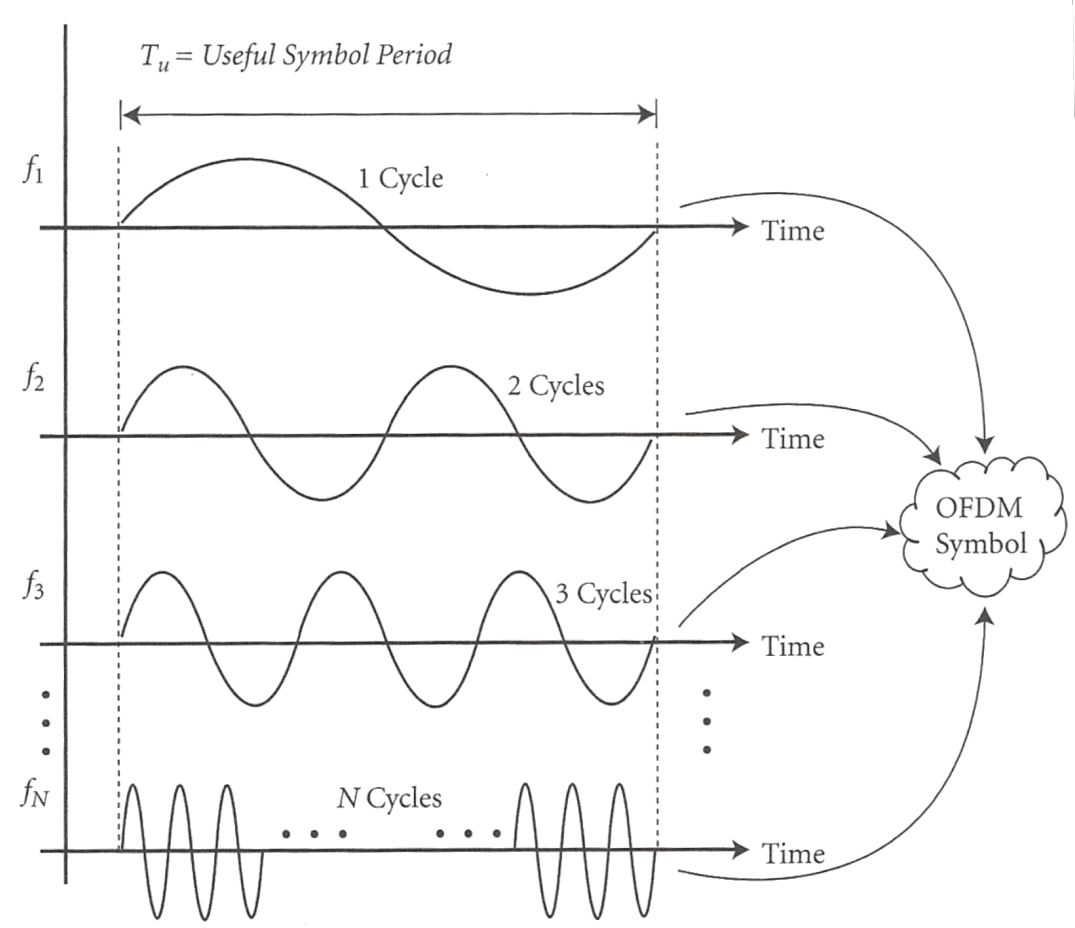
\includegraphics[width=0.5\textwidth]{imgs/ofdm_sinc.png}
\end{center}

Nella figura si può vedere come quando andiamo a trasmettere $s[k] = \sum_{n=0}^{N-1} S_n e^{\frac{j2\pi n k}{N}}$ si vada a trasmettere la combinazione delle seguenti sinusoidi, come rappresentate singolarmente in figura:
\[
    \begin{array}{ll}
        n = 0 \Rightarrow \frac{1}{\sqrt{N}} S_0 e^{j2\pi} \\
        n = 1 \Rightarrow \frac{1}{\sqrt{N}} S_1 e^{j2\pi \frac{k}{N}} \\
        \vdots \\
        n = N-1 \Rightarrow \frac{1}{\sqrt{N}} S_{N-1} e^{j2\pi \frac{N-1}{N} k}
    \end{array}
\]



Quindi si ottiene che la banda occupata da OFDM è la somma di N funzioni sinc, ciascuna centrata in una subcarrier differente.
Inoltre ciò che si può notare è che le varie sinc non interferiscono tra loro nelle subcarrier, infatti in corrispondenza di tali valori solo una sinc risulterà non essere nulla. Per contenere la banda le subcarrier agli estremi non sono utilizzate, in modo che al di fuori della banda a disposizione non vi sia un contributo energetico significativo.
\[
    B_{OFDM} \approx N \cdot \frac{1}{NT_s} = \frac{1}{T_s}
\]
Tale relazione vale solo se si impongono virtual carriers per minimizzare il fenomeno indicato come \textbf{out of band radiation} da parte della sinc.
La banda risulta particolarmente ristretta in quanto non ci sono fattori a moltiplicare $\frac{1}{T_s}$, come avviene utilizzando un RRC. Tuttavia parte della banda risulta non sfruttata in quanto è necessario trasmettere sia il prefisso, sia non utilizzare alcune subcarrier agli estremi, dette \textbf{virtual subcarrier}.


Per quanto riguarda il symbol time, in OFDM si ha la relazione con il symbol time:
\[
    T_{OFDM} = T_s(N+N_{CP}), \quad N_{CP} > L
\]  
% TODO: cos'è L?
Dove $L$ non è noto a priori.
% TODO: ma quindi non utilizziamo nyquist?
Da questo valore si ottiene:
\[
    T_s < \sigma_{\tau} \ll T_{OFDM}, \quad B_s > B_c \gg \Delta f
\]
Ogni subcarrier può considerare il canale \textbf{flat-fading}. Il canale per poter ricevere correttamente il segnale deve essere stimato, e ciò avviene su speciali subcarrier detti \textbf{pilot subcarrier}. Su tali frequenze avviene la trasmissione di simboli noti in modo da ricostruire la risposta del canale. Inoltre per poter ridurre la presenza di rumore la tramissione su tali frequenze avviene con una potenza superiore. In realtà la stima del canale è valida solo sulle frequenze pilotate, per quelle intermedie si effettua un'interpolazione e si ottiene un'approssimazione.
L'efficienza spettrale è ridotta dell'utilizzo di virtual subcarriers, pilot-subcarriers e cyclic prefix:
\[
    R = \left[N - (N_v + N_p) \right]\frac{1}{(N+N_{CP})T_s} = \frac{N - (N_v + N_p)}{(N+N_{CP})} \frac{1}{T_s}
\]



\makeatletter
\pgfkeys{/tikz/semiellipse/.cd,
  width/.initial=2cm,
  height/.initial=1cm,
  fill color/.initial=red,
  fill opacity/.initial=0.5
}
\pgfdeclareshape{semiellipse}{
    % The 'anchor' for positioning the node
    \savedanchor\centerpoint{
        \pgf@x=0pt
        \pgf@y=0pt
    }
    \anchor{center}{\centerpoint}
    \anchor{north}{
        \pgf@x=0pt
        \pgf@y=0.5\ht\pgfnodeparttextbox
    }
    \anchor{south}{
        \pgf@x=0pt
        \pgf@y=-0.5\ht\pgfnodeparttextbox
    }
    \anchor{east}{
        \pgf@x=0.5\wd\pgfnodeparttextbox
        \pgf@y=0pt
    }
    \anchor{west}{
        \pgf@x=-0.5\wd\pgfnodeparttextbox
        \pgf@y=0pt
    }

    % The background path
    \backgroundpath{
        % Get parameters
        \pgfkeysgetvalue{/tikz/semiellipse/width}{\semiw}
        \pgfkeysgetvalue{/tikz/semiellipse/height}{\semih}
        \pgfkeysgetvalue{/tikz/semiellipse/fill color}{\semifillcolor}
        \pgfkeysgetvalue{/tikz/semiellipse/fill opacity}{\semifillopacity}

        % Convert to dimensions
        \pgfmathsetlengthmacro\halfwidth{.5*\semiw}
        \pgfmathsetlengthmacro\halfheight{.5*\semih}
        
        % Draw and fill the semi-ellipse
        \pgfpathmoveto{\pgfpoint{\halfwidth}{0pt}}
        \pgfpatharc{0}{180}{\halfwidth and \halfheight}
        \pgfpathclose % Close the path to form a proper semi-ellipse

        % Fill settings
        \pgfsetfillcolor{\semifillcolor}
        \pgfsetfillopacity{\semifillopacity}
        \pgfusepath{fill,stroke} % Fill and then draw the stroke
    }
}
\makeatother

\resizebox{\textwidth}{!}{
    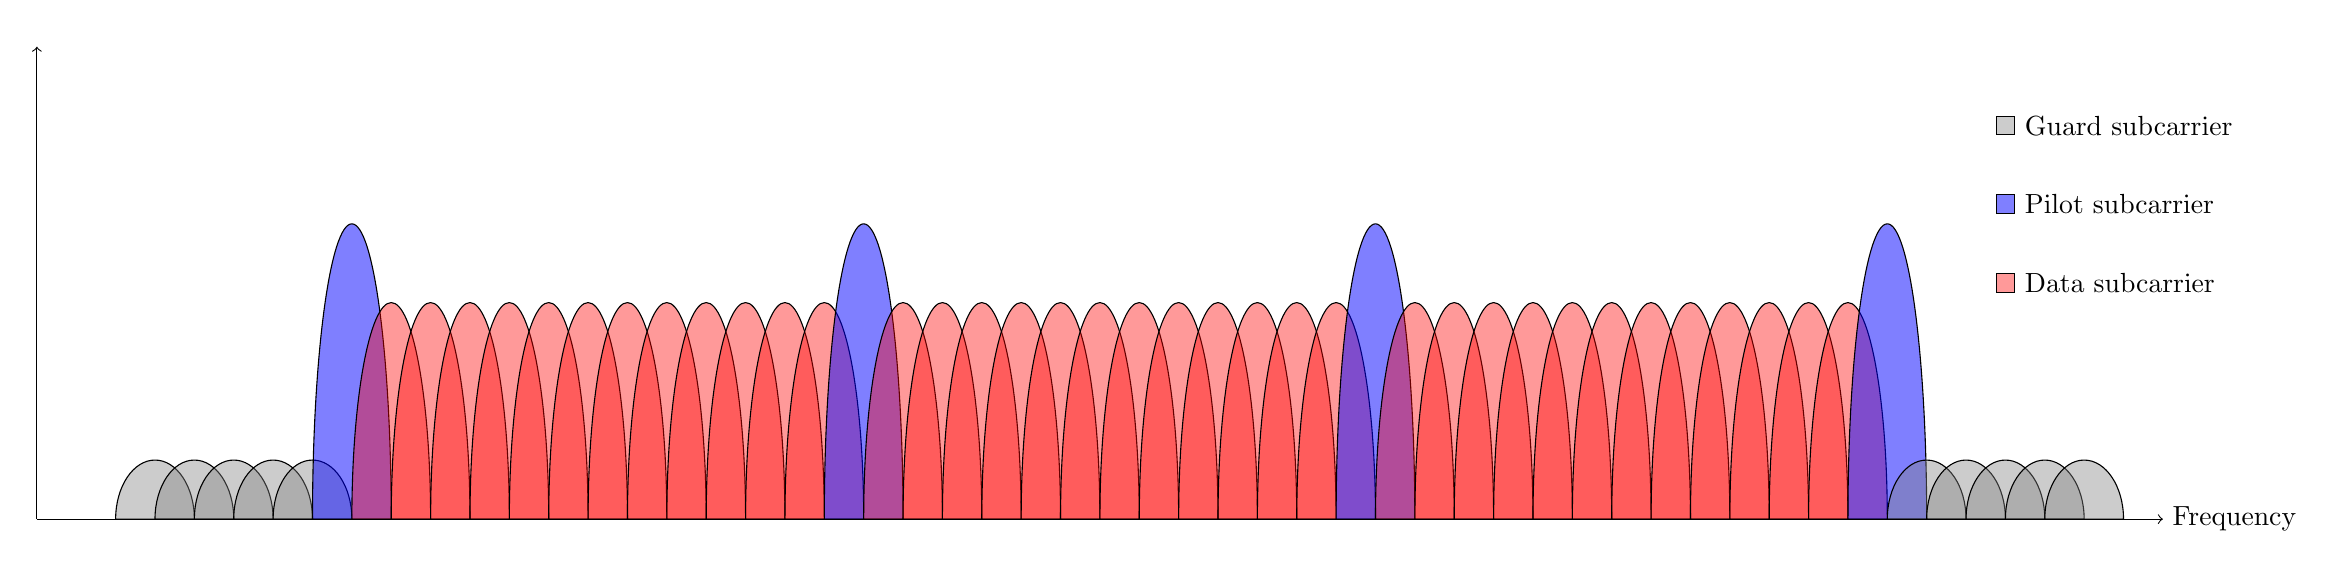
\begin{tikzpicture}    
        \foreach \i in {0,1,2,3,4} {
            \node[shape=semiellipse, draw, semiellipse/width=1cm, semiellipse/height=1.5cm, semiellipse/fill color=gray, semiellipse/fill opacity=0.4] (se) at (0.5+\i*0.5,0) {};
        }
        \node[shape=semiellipse, draw, semiellipse/width=1cm, semiellipse/height=7.5cm, semiellipse/fill color=blue, semiellipse/fill opacity=0.5] (se) at (3,0) {};

        \foreach \i in {7,8,9, 10, 11, 12, 13, 14, 15, 16, 17, 18} {
            \node[shape=semiellipse, draw, semiellipse/width=1cm, semiellipse/height=5.5cm, semiellipse/fill color=red, semiellipse/fill opacity=0.4] (se) at (\i*0.5,0) {};
        }
        \node[shape=semiellipse, draw, semiellipse/width=1cm, semiellipse/height=7.5cm, semiellipse/fill color=blue, semiellipse/fill opacity=0.5] (se) at (9.5,0) {};

        \foreach \i in {19, 20, 21, 22, 23, 24, 25, 26, 27, 28, 29, 30} {
            \node[shape=semiellipse, draw, semiellipse/width=1cm, semiellipse/height=5.5cm, semiellipse/fill color=red, semiellipse/fill opacity=0.4] (se) at (0.5+\i*0.5,0) {};
        }
        \node[shape=semiellipse, draw, semiellipse/width=1cm, semiellipse/height=7.5cm, semiellipse/fill color=blue, semiellipse/fill opacity=0.5] (se) at (16,0) {};
        \foreach \i in {31, 32, 33, 34, 35, 36, 37, 38, 39, 40, 41, 42} {
            \node[shape=semiellipse, draw, semiellipse/width=1cm, semiellipse/height=5.5cm, semiellipse/fill color=red, semiellipse/fill opacity=0.4] (se) at (1+\i*0.5,0) {};
        }
        \node[shape=semiellipse, draw, semiellipse/width=1cm, semiellipse/height=7.5cm, semiellipse/fill color=blue, semiellipse/fill opacity=0.5] (se) at (22.5,0) {};
        \foreach \i in {43, 44, 45, 46, 47} {
            \node[shape=semiellipse, draw, semiellipse/width=1cm, semiellipse/height=1.5cm, semiellipse/fill color=gray, semiellipse/fill opacity=0.4] (se) at (1.5+\i*0.5,0) {};
        }
        \draw[->] (-1,0) -- (26.0,0) node[right] {Frequency};
        \draw[->] (-1,0) -- (-1,6) node[above] {};
        \begin{scope}[shift={(24, 5)}] % Adjust the position of the legend
            \node[draw, fill=gray, fill opacity=0.4, label=right: Guard subcarrier] at (0,0) {};
            \node[draw, fill=blue, fill opacity=0.5, label=right:Pilot subcarrier] at (0,-1) {};
            \node[draw, fill=red, fill opacity=0.4, label=right:Data subcarrier] at (0,-2) {};
        \end{scope}
    \end{tikzpicture}
}




\paragraph*{OFDM error rate}
Considerando la presenza del rumore il segnale ricevuto avrà una componente aggiuntiva di disturbo $\mathbf{n}$, con $\mathbf{n}_k \sim \mathcal{N}(0, \sigma^2), \ \forall k = 0, \ldots, N-1$, quindi il la componente $k$-esima del segnale ricevuto sarà:
\[
    \mathbf{r}_k = \mathbf{y}_k + \mathbf{n}_k
\]
Applicando la DFT si ottiene:
\[
    \mathbf{R} = \mathbf{F}\mathbf{r} = \mathbf{F}\mathbf{y} + \mathbf{F}\mathbf{n} = \mathbf{H}\mathbf{S} + \mathbf{N}
\]

\[
    \mathbf{R}_{m} = \mathbf{H}_{m, m}\mathbf{S}_{m} + \mathbf{N}_{m}
\]
Per poter dare un valore all'errore della modulazione è necessario analizzare le statistiche di $\mathbf{N}_{m}$, ovvero il rumore dopo la DFT.
Data l'unitarietà della matrice $\mathbf{F}$ si ha che le statistiche del rumore dopo la trasformazione rimangono inalterate.
\[
    \mathbb{E}[\mathbf{N}] = \mathbb{E}[\mathbf{F}\mathbf{n}] = \mathbf{F} \mathbb{E}[\mathbf{n}] = \mathbf{0}
\]  
\[
    R_{N,N} = \mathbb{E}[\mathbf{N}\mathbf{N}^H] = \mathbb{E}[\mathbf{F}\mathbf{n}\mathbf{n}^H\mathbf{F}^H] = \mathbf{F}\mathbb{E}[\mathbf{n}\mathbf{n}^H]\mathbf{F}^H = \mathbf{F}R_{n,n}\mathbf{F}^H = \mathbf{F} \sigma^2 \mathbf{I}_N \mathbf{F}^H = \sigma^2 \mathbf{I}_N
\]

Dove $R_{n,n}$ è l'autocorrelazione. Da ciò si ottiene quindi che $\mathbf{N}_{n} \sim \mathcal{N}(0, \sigma^2)$.
Per rimuovere l'effetto introdotto dal canale, ovvero $\mathbf{H}_{m,m}$, il canale è stimato:
\[
    \mathbf{H}_{n, n}= \alpha(n) e^{j\phi(n)}
\]
Se il canale fosse stimato alla perfezione si otterrebbe:
\[
    \mathbf{X}_{n} = \frac{\mathbf{R}_{n}}{\mathbf{H}_{n, n}} = \mathbf{S}_{n} + \frac{\mathbf{N}_{n} e^{-j\phi(n)}}{\alpha(n)}
\]


Se il canale è molto attenuato, ovvero $\alpha(n) \approx 0$, il rumore viene amplificato a seguito della divisione, richiedere un SNR superiore.
La fase non ha alcuna implicazione sul rumore, durante i calcoli di $\sigma ^2=2N_0$ infatti sparisce per via del complesso coniugato.
L'espressione della variabile decisionale è confrontabile con quella di un sistema tradizionale
\[
    x[m] = c_m + n[m] \quad \text{variabile tradizionale}
\]

\[
    \mathbf{X}_{m} = \mathbf{S}_{m} + \mathbf{N}'_{m} \quad \text{variabile OFDM}
\]
\[
    \mathbf{N}'_{m} \sim \mathcal{CN}(0, \frac{\sigma}{\mathbf{H}_{m, m}})
\]
Questo permette di applicare le solite considerazioni per la probabilità di errore:
% TODO: probabilmente non % è H_{m, m}
\[
    \mathbb{P}(e \mid \mathbf{H}_{m, m}) = 2 Q\left( \sqrt{\frac{1}{\sigma^2}}  \right) = 2 Q\left( \sqrt{\frac{E_s \alpha^2(m)}{N_0}}  \right) 
\]
\[
    \mathbb{P}(e) = \sum_{m=0}^{N-1} \mathbb{P}(e \mid \mathbf{H}_{m, m}) \mathbb{P}(\mathbf{H}_{m,m}) = \frac{2}{N} \sum_{m=0}^{N-1} Q\left( \sqrt{\frac{E_s \alpha^2(m)}{N_0}}  \right)
\]

% TODO: qualcosa su OFDMA


\subsection*{WiFi – IEEE 802.11a/g/n/ac}

Una trasmissione WiFi occupa una larghezza di banda \( B = 20 \text{ MHz} \), che è divisa in \( N = 64 \) sotto-portanti spaziate di \( \Delta f = 312.5 \text{ kHz} \). 
La specifica 802.11a/g utilizza 48 sotto-portanti per i dati, 4 per i pilot e 12 come sotto-portanti nulle, mentre la specifica 802.11n/ac utilizza 52 sotto-portanti per i dati, 4 per i pilot e 8 come sotto-portanti nulle.

Il blocco OFDM è composto da \( N = 64 \) campioni e \( N_{CP} = 16 \) campioni di prefisso ciclico (CP). La durata di ogni campione è:
\[
T = \frac{1}{B} = \frac{1}{20 \times 10^6} = 50 \text{ ns}
\]
Pertanto, la durata di un blocco OFDM è:
\[
    T_{OFDM} = (64 + 16) \times 50 \text{ ns} = 4 \si{\mu s}
\]
In generale, il delay spread di un canale interno è \( \sigma_\tau < 500 \text{ ns} \), il che significa che il canale può essere considerato flat fading, cioè:
\[
    \sigma_\tau \ll T_{OFDM}
\]
Assumendo che la mobilità massima interna sia \( v = 3 \text{ m/s} \), per una WiFi a 5 GHz, la massima deviazione Doppler è:
\[
f_d = \frac{5 \times 10^9 \times 3}{3 \times 10^8} = 50 \text{ Hz}
\]
da cui segue che:
\[
T_c = \frac{1}{2f_d} = \frac{1}{2\cdot 50\si{Hz}} = 0.01 \text{ s}
\]
Il canale è quindi considerato slow fading:
\[
T_{OFDM} \ll T_c
\]
Ogni sotto-portante trasporta un nuovo simbolo ogni \( T_{OFDM} = 4 \si{ \mu s} \). La velocità di simboli per sotto-portante è:
\[
\frac{1}{T_{OFDM}} = 0.25 \times 10^6 \si{ simboli/s}
\]
Ci sono 48 sotto-portanti dedicate alla trasmissione dei dati, quindi la velocità complessiva di simboli è:
\[
48 \times 0.25 \times 10^6 = 12 \times 10^6 \si{ simboli/s}
\]
La perdita di efficienza (spettrale ed energetica) dovuta all'inserimento del prefisso ciclico (CP) è:
\[
\eta_{CP} = \frac{N_{CP}}{N + N_{CP}} = \frac{16}{80} = 20\%
\]
Vi è inoltre una perdita aggiuntiva di efficienza spettrale dovuta alle sotto-portanti di guardia e di pilotaggio:
\[
\eta_{GS} = \frac{16}{64} = 25\%
\]
